\documentclass{article}
\usepackage[T1]{fontenc}
\usepackage[scaled=0.95]{helvet}
\renewcommand{\familydefault}{\sfdefault}
\usepackage[paperwidth=16cm,paperheight=7.6cm,margin=0cm]{geometry}
\usepackage{amsmath}
\usepackage{tikz}
\usetikzlibrary{arrows.meta,calc,positioning}
\pagestyle{empty}

\definecolor{ink}{HTML}{0F172A}
\definecolor{muted}{HTML}{64748B}
\definecolor{line}{HTML}{334155}
\definecolor{border}{HTML}{CBD5E1}
\definecolor{paper}{HTML}{F8FAFC}
\definecolor{wash}{HTML}{EEF2FF}
\definecolor{indigo}{HTML}{4F46E5}
\definecolor{violet}{HTML}{7C3AED}
\definecolor{pill}{HTML}{E0E7FF}

\begin{document}
\begin{tikzpicture}[remember picture,overlay,x=1cm,y=1cm,
  >=Latex,
  state/.style={draw=border,fill=white,rounded corners=2.6mm,line width=.45pt,
                minimum width=3.5cm,minimum height=1.78cm,inner sep=0pt},
  latent/.style={draw=none,fill=indigo,rounded corners=5mm,
                 minimum width=1.7cm,minimum height=.86cm,inner sep=0pt},
  action/.style={draw=indigo!55,fill=pill,rounded corners=3mm,line width=.4pt,
                 minimum width=1.75cm,minimum height=.49cm,inner sep=1mm}]
  \coordinate (SW) at (current page.south west);
  \fill[paper] (current page.south west) rectangle (current page.north east);
  \fill[wash] ($(SW)+(0,0)$) circle (2.1cm);
  \fill[indigo!8] ($(SW)+(15.0,6.7)$) circle (1.7cm);

  \node[anchor=west,text=ink,font=\fontsize{15}{17}\selectfont\bfseries]
    at ($(SW)+(0.9,6.82)$) {Intent--JEPA};
  \node[anchor=west,text=muted,font=\fontsize{9.5}{11}\selectfont]
    at ($(SW)+(0.9,6.38)$) {Reasoning evolves through observed language actions};

  \node[state] (s0) at ($(SW)+(2.65,4.82)$) {};
  \node[state] (s1) at ($(SW)+(8.00,4.82)$) {};
  \node[state] (s2) at ($(SW)+(13.35,4.82)$) {};
  \foreach \x/\lab in {2.65/{REASONING STATE $s_t$},8.00/{REASONING STATE $s_{t+1}$},13.35/{REASONING STATE $s_{t+2}$}} {
    \node[text=muted,font=\fontsize{6.4}{7}\selectfont\bfseries] at ($(SW)+(\x,5.39)$) {\lab};
  }
  \node[text=ink,font=\fontsize{14}{15}\selectfont\bfseries] at ($(SW)+(2.65,4.76)$) {$x$ is 8};
  \node[text=ink,font=\fontsize{14}{15}\selectfont\bfseries] at ($(SW)+(8.00,4.76)$) {$y$ is 4};
  \node[text=ink,font=\fontsize{14}{15}\selectfont\bfseries] at ($(SW)+(13.35,4.76)$) {$x\times y=32$};
  \node[text=muted,font=\fontsize{6.5}{7}\selectfont] at ($(SW)+(2.65,4.28)$) {current numerical fact};
  \node[text=muted,font=\fontsize{6.5}{7}\selectfont] at ($(SW)+(8.00,4.28)$) {new fact after execution};
  \node[text=muted,font=\fontsize{6.5}{7}\selectfont] at ($(SW)+(13.35,4.28)$) {derived result};

  \draw[line,line width=1.15pt,->] (s0.east) -- (s1.west);
  \draw[line,line width=1.15pt,->] (s1.east) -- (s2.west);
  \node[action] at ($(SW)+(5.32,5.34)$) {\begin{tabular}{c}\fontsize{5.2}{5.5}\selectfont\color{indigo}\bfseries INTENT ACTION\\[-1pt]\fontsize{6.2}{6.5}\selectfont\color{ink}find value of $y$\end{tabular}};
  \node[action] at ($(SW)+(10.68,5.34)$) {\begin{tabular}{c}\fontsize{5.2}{5.5}\selectfont\color{indigo}\bfseries INTENT ACTION\\[-1pt]\fontsize{6.2}{6.5}\selectfont\color{ink}multiply $x$ and $y$\end{tabular}};

  \foreach \x in {2.65,8.00,13.35} {
    \draw[muted!65,line width=.65pt,dashed,->] ($(SW)+(\x,3.93)$) -- ($(SW)+(\x,2.86)$);
    \node[anchor=west,text=muted,font=\fontsize{5.8}{6}\selectfont\bfseries] at ($(SW)+(\x+0.12,3.29)$) {encode};
  }
  \node[latent] (z0) at ($(SW)+(2.65,2.31)$) {};
  \node[latent] (z1) at ($(SW)+(8.00,2.31)$) {};
  \node[latent] (z2) at ($(SW)+(13.35,2.31)$) {};
  \node[text=white,font=\fontsize{6}{6.5}\selectfont] at ($(SW)+(2.65,2.44)$) {latent state};
  \node[text=white,font=\fontsize{9}{9.5}\selectfont\bfseries] at ($(SW)+(2.65,2.16)$) {$z_t$};
  \node[text=white,font=\fontsize{6}{6.5}\selectfont] at ($(SW)+(8.00,2.44)$) {target state};
  \node[text=white,font=\fontsize{9}{9.5}\selectfont\bfseries] at ($(SW)+(8.00,2.16)$) {$z_{t+1}$};
  \node[text=white,font=\fontsize{6}{6.5}\selectfont] at ($(SW)+(13.35,2.44)$) {target state};
  \node[text=white,font=\fontsize{9}{9.5}\selectfont\bfseries] at ($(SW)+(13.35,2.16)$) {$z_{t+2}$};
  \draw[indigo,line width=1.35pt,->] (z0.east) -- (z1.west);
  \draw[indigo,line width=1.35pt,->] (z1.east) -- (z2.west);
  \node[draw=indigo!45,fill=white,rounded corners=2.5mm,inner sep=1.4mm,text=indigo,
        font=\fontsize{6.2}{6.5}\selectfont\bfseries] at ($(SW)+(5.32,2.55)$) {predictor $F(z_t,a_t)$};
  \node[draw=indigo!45,fill=white,rounded corners=2.5mm,inner sep=1.4mm,text=indigo,
        font=\fontsize{6.2}{6.5}\selectfont\bfseries] at ($(SW)+(10.68,2.55)$) {predictor $F(z_{t+1},a_{t+1})$};

  \node[draw=border,fill=white,rounded corners=2.2mm,minimum width=14.2cm,minimum height=.72cm,
        anchor=south,inner sep=0pt] at ($(SW)+(8.0,.50)$) {};
  \fill[indigo] ($(SW)+(1.30,.88)$) circle (.09cm);
  \node[anchor=west,text=line,font=\fontsize{6.7}{7}\selectfont] at ($(SW)+(1.53,.91)$)
    {\textbf{Observed:} the natural-language intent action};
  \fill[muted!60] ($(SW)+(6.34,.88)$) circle (.09cm);
  \node[anchor=west,text=line,font=\fontsize{6.7}{7}\selectfont] at ($(SW)+(6.57,.91)$)
    {\textbf{Executed:} the environment produces the next reasoning sentence};
  \node[anchor=west,text=muted,font=\fontsize{6.1}{6.5}\selectfont] at ($(SW)+(1.53,.66)$)
    {The model predicts the action-conditioned consequence in latent space; it does not generate the numeric outcome text.};
\end{tikzpicture}
\null
\end{document}
